\documentclass[a4paper]{paper} 
%\usepackage{babel}
\usepackage{hyperref}
\usepackage[margin=2.5cm]{geometry}
\usepackage{pdfpages}
%\usepackage{graphicx}
\graphicspath{{img/}}
\title{Pathfinding on the Lightning Network (with JIT Routing)}
\subtitle{A PhD Proposal - Draft version}
\author{Rene Pickhardt} 
\institution{NTNU Gjovik} 

\begin{document} 
\twocolumn[\maketitle 
\hrule 
\smalltableofcontents
\begin{abstract}
  This PhD proposal follows the structure provided by the Faculty of Engineering Science from the Norwegian University of Science and and Technology (NTNU).
  It suggests to commit 3 years of a PhD study to the path finding problem within privacy aware payment channel networks such as the Lightning Network.
  The path finding problem is non trivial as the topology of privacy aware payment channel networks is only partially known and changes dynamically over time resulting in a non deterministic problem with uncertainty. 
  We propose to create a review of suggested approaches and methods by developing measures to evaluate the quality of path finding methods in such an environment.
  We also propose to collect data about the known topology of the lightning network and probe for less public data.
  Also we suggest to use financial transaction data sets as a basis to evaluate the studied approaches by the scientific method of conducting simulations.
  Furthermore we wish to conduct more experiments to improve and extend the Just In Time Routing schemes (JIT-Routing) which has been proposed by us in early 2019.
  While it can be shown that in its basic form the JIT-Routing heuristic will always improve the routing process it will in its most basic form be economically infeasible for nodes to engage in the JIT-Routing scheme.
  Our goal is to come up with extensions of the scheme that make it viable while keeping almost the same privacy guarantees that privacy aware payment channel networks offer.
  We plan the publication of 3 papers and one technical report to conduct this study. 
The template of this proposal can be found at: \url{https://www.ntnu.edu/documents/139736/20785611/Project+description+-+template+-+English.pdf}
\end{abstract}

\begin{keywords}
Bitcoin, Lightning Network, payment channel networks, path finding, routing, liquidity, flow control, congestion control, game theory, uncertainty, simulations, agent based systems, collaborative problem solving, 
\end{keywords}
\hrule\bigskip
]

\section{Background}
We will address the problem of finding paths in privacy aware payment channel networks such as the Lightning Network.
These peer to peer networks are created in order to allow their participants to route payments through a network of payment channels to another participant.
Usually the unit of account of such payments is some cryptocurrency.
However with stronger data protection regulations like the GDPR and privacy demands by customers even banks might be forced in the future to replace the SWIFT network with a privacy aware payment channel network.
Routing payments through such a network is usually proceeded by finding a path of payment channels so that all channels have enough liquidity to fulfill the forwarding of payments for sending funds from one participant to another one.
As in privacy aware payment channel networks the current liquidity state is kept private to the network a crucial topological information is missing for conducting a traditional path finding algorithm. 
Additionally the already uncertain topology is changing with every payment attempt independently of its success.
The main focus of this PhD project will be to gain a better understanding of how to deal with this uncertainty in order to conduct a successful path finding in such a dynamically changing graph in which only limited topological information is available.
In the very best case one would be able to guarantee the fulfillment of a service level agreement.

As the Lightning Network is the most relevant example of a privacy aware payment channel network we decided to choose it as the leading use case and example throughout our research.
However the applications and results of our research will not be limited to the Lightning Network and could be applied to any other payment channel network such as the Raiden Network.

The Lightning Network became so relevant as it is the most promising approach to scale the amount of payments that can be achieved over the Bitcoin Network.
In its current design every time a participant wants to make a payment she needs to find a path to the recipient such that each link has enough funds to forward the payment.
Theoretically with the Dijkstra Algorithm this is a trivially solved path finding problem in computer science.
In practice the privacy properties of the Lightning Network hide the information about the available liquidity on the existing payment channels (edges) of the network.
Thus crucial topology information is missing and the Dijkstra Algorithm cannot be applied.

To achieve maximal privacy for its users the following cryptographic design decisions have been build into the Lightning Network.
\begin{enumerate}
\item The routing scheme is similar to the sourced based onion routing of the TOR network and utilizes the SPHINX mix format \cite{danezis2009sphinx}
\item Payment channels have a publicly known capacity which is privately spread into a local balance between the two nodes that own the channel. The local balance is not shared with the network. Thus standard path finding techniques known from graph theory cannot be applied directly.
\end{enumerate}

Currently path finding on the Lightning Network is solved by a brute force approach of trying one potential path after another one.
It is easy to see that while probing paths the state of network can change as other payments are conducted successfully.
This could lead to a situation in which a path that was not working on the first attempt might work at a later point in time.

Thus besides uncertainty the problem is highly dynamic and non deterministic.\footnote{If we found a path we would know it exists. But as long as we do not find a path we will not know for sure that no path exists.}
With the desired growth and adoption of the Lightning Network the current path finding strategy does not seem to be feasible.
In particular payments should always be known to succeed or fail within a certain short time period (in the order of at most a few seconds).
While successful path finding seems not sufficient to achieve this goal it seems to be a mandatory requirement to at least be able to give a certain quality assurance or service level agreement.

The White paper of the Lightning Network \cite{poon2016bitcoin} briefly mentions that there could be some TOR like routing scheme applied.
However it is rather vague about the actual routing scheme to be used and does not say a word about path finding techniques.
Already in 2016 Flare \cite{prihodko2016flare} was proposed to fill the void of the white paper.
The approach is using local beacon nodes which oversee the network topology and help to find paths.
The approach of Flare was not persued by the lightning network developers though it seems that a current trends towards trampoline routing\cite{Teinturier2019trampoline} seems to pick up the idea to have an expert overlay network that solves routing decisions for endusers similar to the beacon nodes proposed in Flare.
Ant-routing \cite{grunspan2018ant} was proposed for a Lightning Network which consists only of private channels.
Though it can be shown that the ant scheme will always find a path it will - similarly to the Bitcoin Network - involve every participant of the Network for each payment attempt resulting in poor scaling properties.
Both approaches might be useful if the Lightning Network was designed without a gossip protocol.
However the Lightning Network developers decided to include a gossip protocol\footnote{\url{https://github.com/lightningnetwork/lightning-rfc/blob/master/07-routing-gossip.md}}\footnote{\url{https://bitcoin.stackexchange.com/questions/85264/why-did-the-lightning-network-implement-a-gossip-protocol}} that shares partial information about the topology.
Thus approaches that utilize this information seem more feasible to examine.

The currently most desired approach by the open source community is to use multi path payment schemes \cite{osuntokun2018AMP} which have already been investigated \cite{piatkivskyi2018split} in the scientific literature and have been demonstrated to have a higher success rate than the current approach.
Multi path payment schemes are popular because they do not only help with path finding but also with utilizing the owned liquidity of a participant in the network.
In the past multi path payments have been publicly criticized \cite{pickhardt2019pathfinding} as being too wasteful with resources and yielding the danger of delaying the time to complete of the payment process significantly.
Novel and sophisticated approaches for multi path payments like Boomerang \cite{bagaria2019boomerang} introduce redundant multi path payments to mitigate some of the strongest criticism.
However the Boomerang approach needs either a hard fork to the bitcoin protocol or an extensive extension to the Lightning Network Protocol. 
It was observed that the path finding problem on the Lightning Network might have similarities with path finding in Real Time Strategy games \cite{zmnscpxj2019rts}.

We have proposed Just In Time Routing (JIT Routing) \cite{pickhardt2019jit} which is supposed to get the best effort component into the source base routing process without violating the privacy properties of the Lightning Network.
With JIT Routing a node that is supposed to forward a payment on a channel which does not have enough liquidity can interrupt the routing process and start a local re-balancing operation to provide itself \textbf{just in time} with the needed liquidity before continuing the routing process.
In theory nodes can already implement JIT routing and engage with it without the necessity to have any protocol changes.\footnote{A Basic JIT Routing scheme has recently been implemented by Christian Decker: \url{https://github.com/lightningd/plugins/pull/66}}.
Understanding the mechanics of JIT Routing it is easy to see that as a heuristic it can be included to any other path finding scheme.
In particular it is trivial to see that JIT Routing will never decrease the success rate of a routing attempt.
However in its current form it is believed that JIT-Routing will not be economically feasible for nodes as as they might loose money while engaging in JIT-Routing.
Currenly nodes will try paths starting with the one that takes the cheapest routing fee.
If the rebalancing operation would be cheaper than the fees the node takes for routing the payment that path would have been already tested by the sender to begin with.
This could be mitigated with minor protocol modifications like the addition of fee free circular payments that could be used to rebalancing.
A similar approach was suggested in Revive \cite{khalil2017revive} where groups could rebalance their channels with an open and transparent smart contract that was cryptographically secured.
However the Revive approach needs stronger assumptions to the smart contracting language than the one currently deployed in Bitcoin.
Studying JIT Routing and its dialects, comparing it with other proposed path finding schemes and improving it will be a major goal of the PhD thesis. 

\section{Objectives}
Currently the following research objectives are planned.
\begin{enumerate}
\item Develop a graph theoretic model, framework and notation which can be used to express approaches for path finding in privacy aware payment channel networks.
\item Find measures from the model to classify and compare existing as well as yet to be introduced path finding techniques. A preliminary list of such measures might include: Success rate, interactivity (with other nodes), information need, privacy, time to complete a payment, run time, memory consumption, protocol compatibility, service level agreement,\dots
\item Work out the difficulties and trade offs which exist in path finding. The most obvious trade off seems to be the trade off between privacy and success rate\footnote{Probably even the ability to deterministicly guarantee that a path can be found.}.
\item Study and understand if path finding can be solved when we seek for privacy, scalablity and want to support a dynamically changing network or if one has to drop at least one requirement. 
\item In particular we want to study the JIT Routing scheme and potential enhancements of it. We first want to inspect a node that supports JIT routing to demonstrate that the current approach would improve the routing successrate over the network despite being economically infeasible.
\item We suppose that backward compatible and rather small protocol changes like local information sharing of channel balances and fee free re-balancing operations would significantly increase the usefulness of JIT Routing. This shall be investigated in a second study about JIT-Routing. 
\item Make educated suggestions which path finding techniques seem most promising.
\end{enumerate}


\section{Scope}
We will use simulations of payments within the lightning network and statistical evaluation as the main research method to study and compare the existing approaches.
In order to do so we need three types of experimental data:
\begin{enumerate}
\item The topology of the lightning network which is publicly available via the gossip protocol. In combination with the data from the Bitcoin blockchain we can even predict who opened the channel and thus know the initial balance of each payment channel.
\item A data set of payments between participants in a payment network. While it would be possible to set up several lightning nodes to collect actual data on the lightning network this would require quite some Bitcoin and financial risk.\footnote{It might be possible to talk to liquidity providers such as LNBIG or ACINQ if they would be willing to share some data that they have collected.} It seems more realistic to use the public data set from the Kaggle\footnote{\url{https://www.kaggle.com/}} as has been done in the past \cite{sivaraman2018routing}. 
\item In order to have a good baseline it makes sense to not only simulate the currently used approaches with our synthetic data set but collect some data from our own lightning node by making payment attempts to other participants.\footnote{By paying to fake payment hashes one can simulate the success of such payments without actually sending money to other nodes}. This data set can be used to gauge the results from the simulations on the synthetic payment data set.
\end{enumerate}

The simulation will be limited to a turn based simulation of payments instead of a concurrent setup.
However turns can be much shorter than one payment process so that at least partially the realistic behavior of concurrent payments will be modeled.

Another dataset comes from the logfiles of the node that runs the JIT-Routing scheme.
We will measure how much we paid for the rebalancing in comparision to the routing fees to see if the simple JIT Routing is in fact economically infeasible.

The bigger picture of this research is to improve the payment process and user experience of the Lightning Network.
Path finding seems to be a mandatory requirement to achieve this.
Yet other extensions of the Lightning Network such as cancelable and stuckless payments\cite{gondo2019stucklss} will most likely be necessary too.
As these proposals are related to the cryptographic protocols of the Lightning Network they are explicitly excluded from this research.

While we would be delighted if we solved the general path finding or even the payment problem in privacy aware payment channel networks we will not aim for this goal as it seems far to complex for a PhD thesis.
Also it might be interesting to study the dynamic topological changes of privacy aware payment channel networks themselves.
Even though this information might be possible to collect we do not plan to focus our activities in this direction at this point.

\section{Expected results}
We expect to gain a deeper understanding of how to handle uncertainty in privacy aware payment channel networks.
In particular we will understand what additional information is necessary to make JIT-Routing a useful path finding scheme. 
In the best case we will be able to demonstrate the superiority of a certain path finding scheme or even come up with one by using the insight from our research.
As there are several companies building the Lightning Network Protocol and software and as there is heavy open source development on the Mailing list\footnote{\url{https://lists.linuxfoundation.org/pipermail/lightning-dev/}} and in the git repositories \footnote{\url{https://github.com/lightningnetwork/lightning-rfc}} we expect that the results will be picked up by the open source community and industry.

\section{Work plan/work schedule}
While it would be nice if the research objectives could be achieved in a linear way one after another we do not expet this to happen.
For example developing proper models, frameworks and notation seems to be an iterative process which will be refined over the time and with experience.

We will start our research with a survey article of path finding techniques in the lightning network.
This should not take more than the first year and will be used to achieve the first two objectives (modeling, measuring and coming up with a taxonomy).

In parallel we will start to collect and clean the data that will be necessary to do the planed experiments.
This will in particular include the temporal evolution of the known topology information of the Lightning Network.
The data collection process is probably ongoing during the remainder of the PhD program.
In the best case it will just require a little bit of monitoring.
However we plan some buffer time every quarter for unforeseeable protocol changes that allow other data to be collected or which need to happen with implementation changes.

As soon as we finished our survey we will be able to finalize our simulation framework and conduct experiments that utilize the collected data and compare the various path finding techniques.

In particular we will be able to start the experiments regarding JIT routing.
An earily step will be to enable JIT-Routing on a Lightning Network node so that we can collect data about the usage of JIT Routing even if we have to subsidise the algorithm by paying more for the rebalancing fees than we earn by routing the payments.

Having all this information and experience we will be able to fully analyze and study how JIT-Routing schemese need to be deployed to be as useful as possible.
The study about refining the JIT-Routing schemes will lead to our last publication.
Everything will be summarized in the dissertation and defense at the end (: 

As the Lightnining Network is the most prominant example of a payment channel network and most research is connected to the development of the Lightning Network we will also regularly spend time to participate in the Lightning Network Open Source community.
New ideas are proposed, shared and discussed over the lightning-dev mailinglist\footnote{\url{https://lists.linuxfoundation.org/pipermail/lightning-dev/}}.
The ongoing specification work of the protocol takes place in the lightning-rfc git repository \footnote{\url{https://github.com/lightningnetwork/lighting-rfc}}.
In order to keep track of new ideas and proposals but also to successfully dissiminate our results we will closely follow and contribute the lightning network devleoper community on a regular basis during the PhD program with roughly 15 \% of our time.

A more detailed overview of the allocated time can be found at the end of the document in the table.

\bibliography{proposal}
\bibliographystyle{plain}

\appendix
\section{Background on Bitcoin and the Lightning network}
The application of Hashcash \cite{back2002hashcash} - better known as proof of work -  has lead to the emergence of decentralized digital currencies such as Bitcoin\cite{nakamoto2008bitcoin}.
Decentralization is achieved by replicating the ledger of all previously agreed upon transactions to all participants of the network.
This ledger is referred to as the blockchain.
This design in combination with the difficulty adjustment of the proof of work system prevent scaling of peer to peer networks such as the Bitcoin Network even when adding more computational resources.

The commonly agreed upon approach to achieve a higher amount of payments is by working off chain.
Instead of storing all payments as transactions to the common, replicated ledger users will only store special transactions that - with the help of smart contracts - open a payment channel.
The payment channels can form a network.
With the help of hashed time locked contracts payments can theoretically be routed from any participant in the network to any other participant. 

The Lightning Network is the most prominent and wide spread example of such a payment channel network.
We will only work with publicly announced channels and assume that the Lightning Network only consists of publicly known channels.


\null\newpage
\begin{minipage}[t]{0.8\linewidth}
  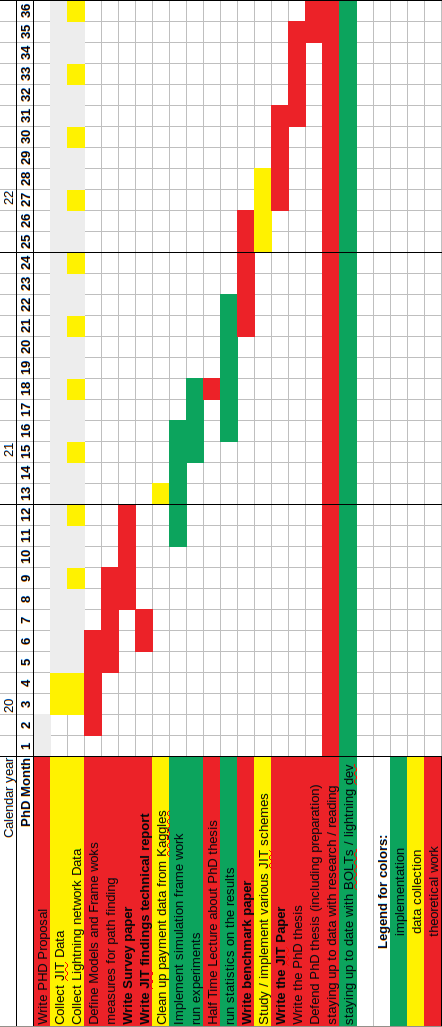
\includepdf[scale=0.85,pagecommand={},linktodoc=true]{timeline.png}
\end{minipage}





\end {document}

